%!TEX root = ../effc_top.tex

\begin{frame}[fragile]{Operations at odd primes}
	\pause
	Steenrod squares come from the symmetry of the \textbf{binary} diagonal.

	\medskip\pause
	Steenrod, and more generally May, also defined operations
	\[
	P_k \colon H^\bullet(X; \Fp) \to H^\bullet(X; \Fp)
	\]
	from the symmetry of diagonal $X \to X \times \dots \times X$.

	\medskip\pause
	\colorit{Note}: indirect group homology definition.
	No generalizations of cup-$i$.

	\bigskip\pause
	\colorit{Construction (Kaufmann-Med.)} \\
	Explicit cup-$(p,i)$ coproducts defining these operations.

	\medskip\pause
	\colorit{Example} \\
	Using the computer algebra system \colorit{\texttt{ComCH}} we have $\Delta_{3,2}[0,1,2] = $

	\begin{verbatim}
		- [0,1][0,1,2][0,1] + [0,1,2][0,2][0,1] + [0,2][0,2][0,1,2]
		- [0,1,2][0,1,2][1] - [0,2][0,1,2][1,2] + [0,1,2][1,2][1,2]
		- [0,1][1,2][0,1,2] - [0,1,2][2][0,1,2] - [0][0,1,2][0,1,2]
	\end{verbatim}
\end{frame}

\begin{frame}{A more abstract viewpoint}
	\pause
	Operads control algebraic structures.

	\bigskip\pause
	The operad $\mathcal{C}om$ controls cocommutative and coassociative coalgebras.

	\bigskip\pause
	An $E_\infty$-operad is an $\Sym$-cofibrant resolution of $\mathcal{C}om$.

	\bigskip\pause
	Controls coalgebras cocomm. and coassoc. up to coherent homotopies.

%	\bigskip\pause
%	$E_\infty$-structures have a long history:
%	\smallskip\pause
%	\begin{itemize}
%		\item (co)homology operations,
%		\item recognition of infinite loop spaces,
%		\item algebraic models of the homotopy category.
%	\end{itemize}

	\bigskip\pause
	\colorit{Fact}:
	Fully deriving its diagonal map, the chains of a space form an $E_\infty$-coalgebra.

	\bigskip\pause
	\colorit{Principle} (Quillen, Sullivan, Mandell, ...): \\
	\textbf{All} homotopy information of spaces is in this algebraic model.

	\bigskip\pause
	\colorit{Question}: How explicit can this $E_\infty$-structure be made?
\end{frame}

\begin{frame}{Explicit $E_\infty$-structure on (co)chains}
	\pause
	\colorit{Theorem (Med.)} \\
	The collection of maps $\gchains(\gsimplex^n) \to \gchains(\gsimplex^n)^{\otimes r}$ obtained from compositions of
	\begin{align*}
		\Delta &\colon \gchains(\gsimplex^n) \to \gchains(\gsimplex^n)^{\otimes 2}
		\qquad \text{(AW diagonal)} \\
		\ast &\colon \gchains(\gsimplex^n)^{\otimes 2} \to \gchains(\gsimplex^n)
		\qquad \text{(Join map)}
	\end{align*}
	defines an $E_\infty$-coalgebra on simplicial chains.

	\bigskip\pause
	\colorit{Join map} \\
	\qquad\qquad \scalebox{0.7}{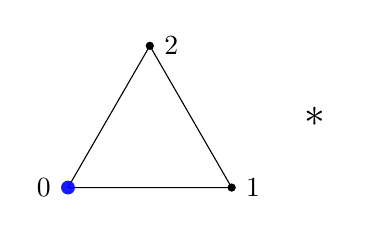
\begin{tikzpicture}[scale=.6]
\coordinate (A) at (210:2);
\coordinate (B) at (-30:2);
\coordinate (C) at (90:2);

\draw[draw=black] (A) -- (B) -- (C) -- (A);

\node[circle,fill=blue, opacity=.9, inner sep=0pt,minimum size=5pt, label=left:{0}] (a) at (A) {};
\node[circle,fill=black,inner sep=0pt,minimum size=3pt, label=right:{$1$}] (a) at (B) {};
\node[circle,fill=black,inner sep=0pt,minimum size=3pt, label=right:{$2$}] (a) at (C) {};

\node[scale=1.5] at (3.5,0.5) {$\ast$};
\end{tikzpicture}
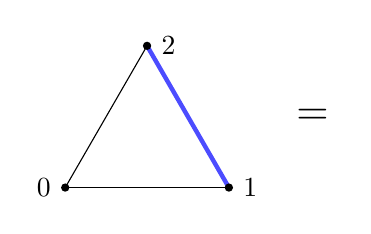
\begin{tikzpicture}[scale=.6]
\coordinate (A) at (210:2);
\coordinate (B) at (-30:2);
\coordinate (C) at (90:2);

\draw[draw=blue,  ultra thick, draw opacity=.7] (B) -- (C);
\draw[draw=black] (C) -- (A);
\draw[draw=black] (A) -- (B);

\node[circle,fill=black,inner sep=0pt,minimum size=3pt, label=left:{$0$}] (a) at (A) {};
\node[circle,fill=black,inner sep=0pt,minimum size=3pt, label=right:{$1$}] (a) at (B) {};
\node[circle,fill=black,inner sep=0pt,minimum size=3pt, label=right:{$2$}] (a) at (C) {};

\node[scale=1.5] at (3.5,.5) {=};
\end{tikzpicture}
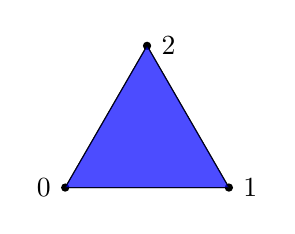
\begin{tikzpicture}[scale=.6]
\coordinate (A) at (210:2);
\coordinate (B) at (-30:2);
\coordinate (C) at (90:2);

\draw[draw=black] (A) -- (B) -- (C) -- (A);

\node[circle,fill=black,inner sep=0pt,minimum size=3pt, label=left:{$0$}] (a) at (A) {};
\node[circle,fill=black,inner sep=0pt,minimum size=3pt, label=right:{$1$}] (a) at (B) {};
\node[circle,fill=black,inner sep=0pt,minimum size=3pt, label=right:{$2$}] (a) at (C) {};

\draw[draw, fill=blue, opacity=.7] (A) -- (B) -- (C) -- (A);
\end{tikzpicture}}

	\bigskip\pause
	\colorit{Other versions} \\
	\colorit{1)} Cubical (Kaufmann--Med.) \\
	\colorit{2)} Multisimplicial (Med.--Pizzi--Salvatore).
\end{frame}

\begin{frame}{A finitely presented $E_\infty$-prop}
	\pause Consider the prop $\cM$ generated by
	\[
	\begin{tikzpicture}[scale=.4]
		\draw (0,.5)--(0,-.75);
		\node[scale=.5] at (0,.75){1};
		\fill (0,-.65) circle (3pt);
	\end{tikzpicture}
	\qquad
	\begin{tikzpicture}[scale=.4]
		\draw (0,0)--(0,.75);
		\draw (0,0)--(.5,-.5);
		\draw (0,0)--(-.5,-.5);
		\node[scale=.5] at (-.5,-.75){1};
		\node[scale=.5] at (.5,-.75){2};
	\end{tikzpicture}
	\qquad
	\begin{tikzpicture}[scale=.4]
		\draw (0,0)--(0,-.75);
		\draw (0,0)--(.5,.5);
		\draw (0,0)--(-.5,.5);
		\node[scale=.5] at (-.5,.75){1};
		\node[scale=.5] at (.5,.75){2};
	\end{tikzpicture}
	\vspace*{-2pt}
	\]
	in degrees $0, 0$ \& $1$ with non-zero boundary
	\[
	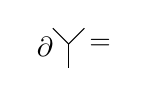
\begin{tikzpicture}[scale=.4]
		\node[scale=1] at (-.75,-.1){$\partial$};
		\draw (0,0)--(0,-.75);
		\draw (0,0)--(.5,.5);
		\draw (0,0)--(-.5,.5);
		\node[scale=1] at (1,0){$=$};
	\end{tikzpicture}
	\begin{tikzpicture}[scale=.4]
		\draw (0,.5)--(0,-.75);
		\fill (0,-.65) circle (3pt);
		\draw (.5,.5)--(.5,-.75);
		\node[scale=1] at (1.15,0){$-$};
	\end{tikzpicture}
	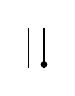
\begin{tikzpicture}[scale=.4]
		\draw (0,.5)--(0,-.75);
		\fill (.5,-.65) circle (3pt);
		\draw (.5,.5)--(.5,-.75);
	\end{tikzpicture}
	\]
	\vskip-5pt
	and relators
	\[
	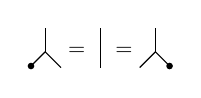
\begin{tikzpicture}[scale=.4]
		\draw (0,0)--(0,.75);
		\draw (0,0)--(.5,-.5);
		\draw (0,0)--(-.5,-.5);
		\fill (-.45,-.45) circle (3pt);
		\node[scale=.8] at (1,0){$=$};
		\draw (1.75,.75)--(1.75,-.5);
		\node[scale=.8] at (2.5,0){$=$};
		\draw (3.5,0)--(3.5,.75);
		\draw (3.5,0)--(4,-.5);
		\draw (3.5,0)--(3,-.5);
		\fill (3.95,-.45) circle (3pt);
	\end{tikzpicture}
	\quad\qquad
	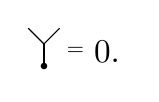
\begin{tikzpicture}[scale=.4]
		\draw (0,0)--(0,-.75);
		\draw (0,0)--(.5,.5);
		\draw (0,0)--(-.5,.5);
		\fill (0,-.7) circle (3pt);
		\node[scale=.8] at (1,-.25){$=$};
		\node[scale=1.2] at (2,-.25){$0.$};
	\end{tikzpicture}
	\]

	\medskip\pause
	\colorit{Theorem (Med.)} \\
	The operad associated to $\Med$, defined by
	\[
	\forget(\cM) = \{\cM(1,r)\}_{r \geq 1},
	\]
	is a (cofibrant and Hopf) $E_\infty$-operad.
\end{frame}